%\documentclass[11pt]{report}
%\usepackage{siunitx}
%\usepackage{graphicx}
%\usepackage{amsmath}

%\begin{document}
%\setcounter{chapter}{2}
%\tableofcontents


\newpage
\chapter{Numerical modelling of mechanical stimulation}
This chapter contains the results of the numerical modelling approaches applied to perfusion setups to predict fluid flow-induced shear stress. This chapter's contents were compiled from the following published works:
\begin{itemize}
\item \small \textit{Meneses, João, João C Silva, Sofia R Fernandes, Abhishek Datta, Frederico Castelo Ferreira, Carla Moura, Sandra Amado, Nuno Alves, and Paula Pascoal-Faria. 2020. “A Multimodal Stimulation Cell Culture Bioreactor for Tissue Engineering: A Numerical Modelling Approach.” Polymers 12 (4)};
\item \small \textit{Meneses, João, Sofia R. Fernandes, Abhishek Datta, Sandra Amado, Nuno Alves, and Paula Pascoal-Faria. 2022. “Numerical Modelling of a Bioreactor Design Targeting Optimal Conditions for Cell Culture.” AIP Conference Proceedings 2425 (1): 220003};
\end{itemize}
\newpage




\section{Introduction}

Mechanical stimulation can be applied to \textit{in vitro} cell cultures in multiple ways, as described in both Chapters 1 and 2. One of the most typical mechanical stimulation systems is a stretching/compression setup that directly applies tensile strain to the cell adhesion substrate, for example, to the scaffold material. These setups can be applied by different actuators, like systems that use a vacuum to deform elastic membranes where cells had previously adhered \cite{Wang2017-bk}, or systems that use pistons to compress cell scaffold structures \cite{Schreivogel2019-ec, Friedl2007-ux, Sandino2008-fn}. Numerical models of stretching/compressing external stimulation systems are extensively reviewed by Vetch \textit{et al.} \cite{Vetsch2015-xz}. Other kinds of systems that apply mechanical stimulation are vibration setups that generate low-level vibrations employing electromagnetic actuators controlled by function generators, like the system applied by Gao \textit{et al.} \cite{Gao2017-pn}, for which examples of numerical models in the literature were not found. Also in this category, ultrasound setups use a sonicator device to deliver oscillatory perturbations to the cell culture region \cite{Liu2022-kf, Uddin2013-xh}, where the impact and magnitude of the delivered stimulus can be predicted, for example, with the developed \ac{FEM} techniques and computational mechanobioregulatory models \cite{Grivas2019-ab}. Another way of applying mechanical stimulation to \textit{in vitro} cell cultures is to use hydrostatic pressure, where this kind of setup applies pressure transients to the entire cell culture chamber \cite{Henstock2013-co, Nesler2016-le, Stavenschi2018-ze}. In those pressure setups, numerical model implementations of \ac{CFD} are used to predict the described pressure fluctuations accurately. These models are also used to predict the fluid flow-induced shear stress generated by the interaction between perfusing culture medium fluid and the cellular/scaffold/bioreactor bodies \cite{Hidalgo-Bastida2012-tp}. The mechanical stimulation applied by perfusion setups works by controlling the culture medium flow velocity \cite{Banka2012-uo}, and its model predictions at the cell culture region may further be combined with mechano-regulation theory to optimize flow rates and cell culture outcomes \cite{Zhao2018-ci}, leading in turn to more efficient cultures. 

As described in Chapter 2, this thesis focuses on perfusion bioreactors, since they can create dynamic cell culture conditions that facilitate mass transport and waste removal to/from the cells. While performing this task with perfusion, bioreactors simultaneously apply a fluid flow-induced shear stress and/or hydrostatic pressure that will act as a mechanical stimulus to cultured cells \cite{McCoy2010-hy, Bhaskar2018-cr, Beskardes2018-fq, Lovecchio2019-ut, Sart2016-uq}. In this chapter, \ac{CFD} models were applied to a developed multimodal perfusion bioreactor design (capable of simultaneous electrical and mechanical stimulation), to find the inlet fluid velocity magnitude that, according to the literature, can be predicted to generate a shear stress range capable of promoting osteodifferentiation of \ac{MSCs} \cite{Zhao2018-ci}. 

Once the inlet fluid velocity is calculated, a precise application of this fluid flow is required to deliver a precise \ac{WSS} range. Different pumps from different manufacturers pose a challenge since these include different tube diameters and specific built-in characteristics that result in different output flow rates. To address the application of perfusion with velocity-limiting laboratory equipment, a \ac{CFD} model was used to adapt the current bioreactor design to a specific perfusion protocol and a specific peristaltic pump. The proposed bioreactor is also ready to be radially expanded, so it can accommodate scaffolds capable of filling large bone defects. All bioreactor parts were designed considering all constraints and requirements for fabrication by a commercially available fused deposition modelling \ac{3D} printer. 

Along the described work a strict relationship was established between the design and numerical prediction phases, iterating through multiple designs until they culminate in the presented solution proposals.



\section{Aims}
The work described in this chapter has the following main goals:
\begin{itemize}
\item Numerical modelling a new perfusion bioreactor design (compatible with additive manufacturing requirements) to predict the fluid flow inlet velocity parameters that generate optimal fluid flow-induced shear stress stimulation at the cell culture region, within a range of  reported \textit{in vitro} osteogenic values;
\item Numerical modelling of perfusion bioreactor design variations concerning the flow path and channel dimensions, to adapt the design for an established osteoinductive shear stress to be achieved, considering the use of limiting peristaltic pump equipment.
\end{itemize}




\section{Methods}

\subsection{Design of a perfusion bioreactor}
A cylindrical perfusion bioreactor was developed to achieve a uniform fluid flow in the cell culture region (bioreactor center). The bioreactor design is presented in Figure \ref{figReactorA}. It contains two symmetric inlets opposed 180\si{\degree} from each other and four outlets disposed radially at the region of cell culture (Figure \ref{figReactorA}a, \ref{figReactorA}b). One flow splitter was added between each inlet and the scaffold to prevent the inlet flow from directly colliding with the scaffold, establishing indirect flow prevalence in the culture region (Figure \ref{figReactorA}a). The radial outlet system was designed to ensure that the fluid exiting from every outlet branch converges into a single outlet going through the same distance, thus keeping the fluid pressure drop homogeneous among all four outlet branches (Figure \ref{figReactorA}b). Each inlet and outlet has a hose joiner for connection with tubes to the peristaltic pump system. The cell culture chamber is divided into two parts to allow the placement and removal of the cell culture scaffold and the cell seeding process.  The scaffold structure is kept entrapped between the top and bottom parts. This perfusion bioreactor was designed using SOLIDWORKS 2018 Student Edition (Dassault Sistèmes). The final design version was exported to the \acs{STEP} format for further \ac{FEM} analysis.

An electrical stimulation apparatus was added to the designed perfusion bioreactor (already capable of mechanical stimulation through fluid flow-induced shear stress), introducing the parts required to achieve a multimodal bioreactor. This electrical stimulation apparatus was included to account for its overall impact in the full bioreactor geometry, which translates into changes in the resultant fluid flow. Electrodes were embedded into each fluid flow splitter component. Each electrode reserved space allows for a circular electrode shape with a diameter of 6 \si{\milli\meter}, placing the two electrodes 16 \si{\milli\meter} apart (Figure \ref{figReactorA}a). The parallel plate capacitor geometry was selected for our design because it predictably results in an electric field distribution with uniform magnitude and primary orientation defined by the direction perpendicular to the electrode plate surfaces \cite{Sherman1982-jz}.

\begin{figure}
\makebox[\textwidth][c]{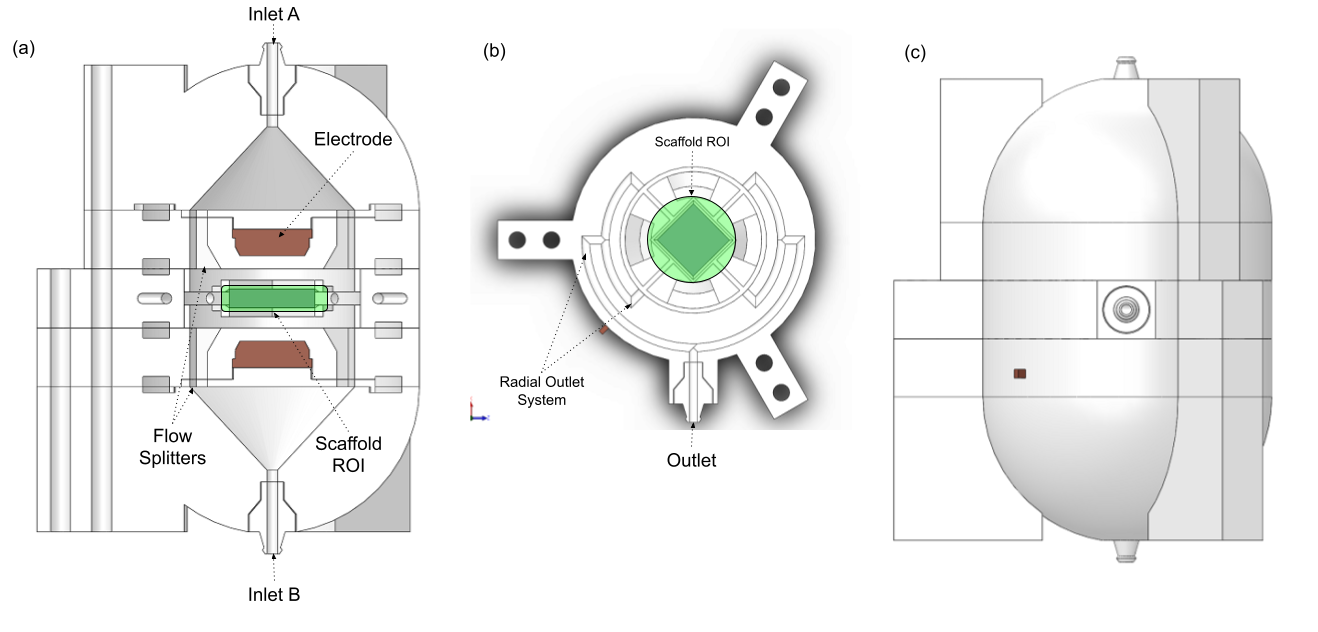
\includegraphics[scale=0.35]{./figures/Figure_3d1}}
\caption{Novel bioreactor design: (\textbf{a}) Vertical cut view of the bioreactor design with parallel electrodes setup, the upper and bottom inlets, and the inlet flow splitters can be observed. (\textbf{b}) Horizontal cut view of the bioreactor design, where the radial outlet system can be observed. The green regions represent the \ac{ROI} where the scaffold and/or cell culture will be placed. This region was represented by a cylinder with a height of 4 \si{\milli\meter} and a diameter of 10 \si{\milli\meter}. (\textbf{c}) Bioreactor \ac{CAD} design assembled in frontal view, the outlet hose joiner is visible in the middle.}
\label{figReactorA}
\end{figure}   


\subsection{Modelling osteogenic promoting perfusion flow}

\ac{FEM} modelling was performed using the \ac{CFD} module from COMSOL Multiphysics software (version 5.2a, Stockholm, Sweden). A stationary study was performed with the \textit{Laminar Flow (spf)} physics interface, solving the equations for a single-phase incompressible fluid in the laminar flow regime, i.e. the Navier-Stokes equations for conservation of momentum and the continuity equation for conservation of mass (equations \ref{NS1}, \ref{NS2}, \ref{NS3}). 

\begin{equation}
\label{NS1}
\nabla \cdot u = 0
\end{equation}

\begin{equation}
\label{NS2}
\rho \frac{\partial u}{\partial t} + \rho u \cdot \nabla (u) = -\nabla p + \nabla \cdot (\mu (\nabla u + \nabla u^T)) + F
\end{equation}

\begin{equation}
\label{NS3}
\rho C_p \frac{\partial T}{\partial t} + \rho C_p u \cdot \nabla T = \nabla \cdot (k \nabla T) + Q
\end{equation}

\noindent were $u$ is the velocity field, $p$ represents the pressure, and $T$ the temperature of the fluid in the modeled domain. $F$ is the Navier-Stokes equation term that represents the external forces applied to the fluid. $\rho$ is the fluid kinematic viscosity, $k$ is the thermal conductivity of the fluid, $C_p$ is the specific heat, and $Q$ represents dissipation. Navier-Stokes equations follow the principle of conservation of the energy, momentum, and mass of a fluid flow. 

Our goal was to find which input stimulation fluid velocity originated proper osteogenic \ac{WSS} values. Osteogenic flow stimulation conditions were reported, for example, in experimental studies conducted by Zhao \textit{et al.} \cite{Zhao2018-ci}. Zhao \textit{et al.} work found that the optimal flow rates, under which the highest fraction of scaffold surface area is subjected to a wall shear stress that induces mineralization, are strongly dependent on the scaffold geometries. Nevertheless, the variation range of such optimal flow rates was found to be within 0.5 to 5 \si{\milli\liter\per\minute} (or fluid velocity: 0.166--1.66 \si{\milli\meter\per\second}). Those ranges were obtained considering different scaffold geometries and predictions from a mechano-regulation theory, where extracellular matrix mineralization would be stimulated with \ac{WSS} values previously reported as being osteogenic \cite{Zhao2018-ci}.

\begin{figure}
\makebox[\textwidth][c]{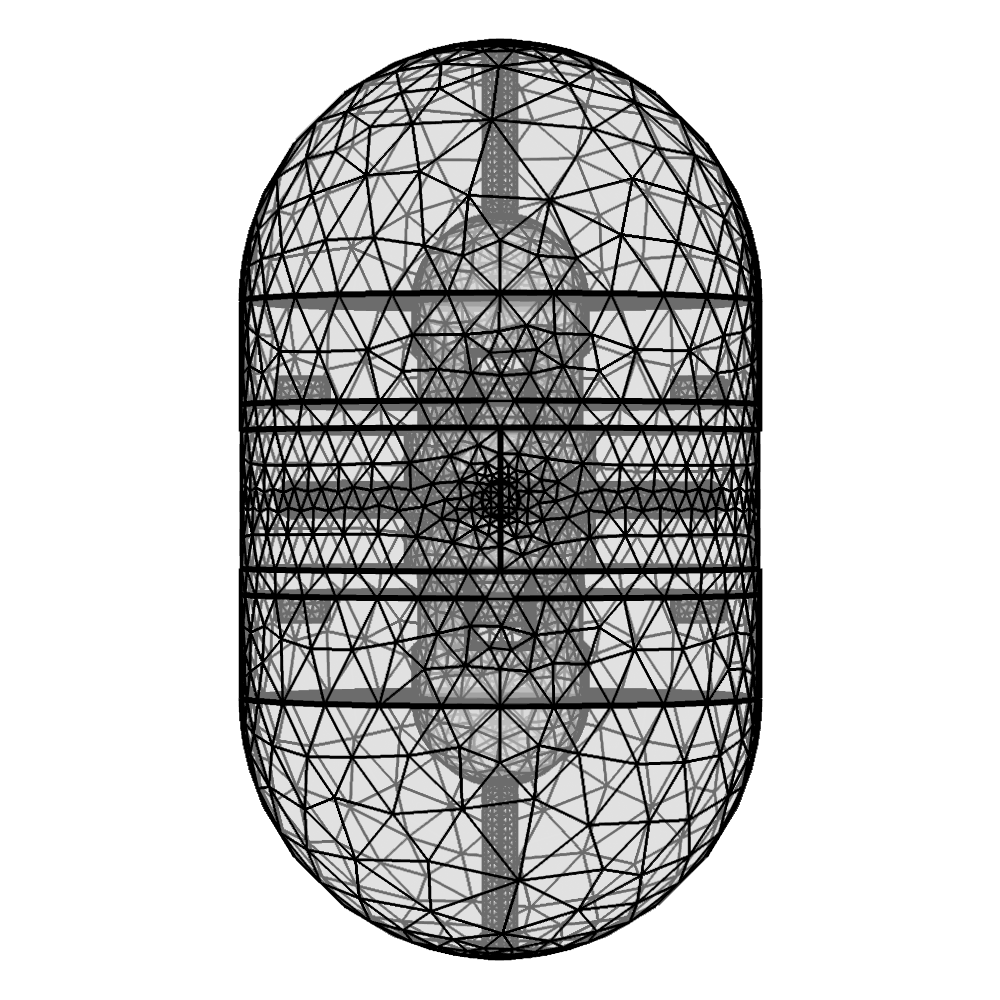
\includegraphics[scale=0.6]{./figures/Figure_3d2}}
\caption{Bioreactor geometry volume mesh created using COMSOL Multiphysics, with 1.9 $\times$ 10$^{6}$ elements and an average element quality of 0.65. External connector parts were excluded from \ac{FEM} analysis.}
\label{figMesh}
\end{figure}   

The \ac{CAD} model of the bioreactor was imported into COMSOL, where a physics-controlled mesh was generated with \num{1.9d6} tetrahedral volume elements and an average element quality of 0.65, as shown in Figure \ref{figMesh}. The final geometry comprised two distinct domains: one fluidic domain, made from culture medium material, and one construction domain, consisting of \acs{PETG} material. The temperature for this simulation was set at 37 \si{\degreeCelsius}. Regarding the COMSOL laminar flow study, the fluid domain representing the culture medium was assumed to be a homogeneous and incompressible Newtonian fluid with a volume density of 993.3 \si{\kilo\gram\per\cubic\meter} and dynamic viscosity of \num{6.9d-4} \si{\pascal}$\cdot$\si{\second}. Considering that the \acs{ROI} diameter is 0.010 \si{\meter}, and the fluid velocity in the same region was established at 0.0016 \si{\meter\per\second} \cite{Zhao2018-ci}, the calculated Reynolds number was 18.51, which is less than the threshold for turbulent flow (2300) \cite{Chen2019-cl}, so a single-phase laminar flow regime was also considered. The \ac{GMRES} solver was selected with adaptive meshing for local solution improvement. Boundary conditions were set for all bioreactor's walls with a no-slip condition. This boundary condition is valid for low-viscosity fluids at all fluid-solid boundaries, meaning that the fluid velocity is considered zero at the surface interface, starting to increase in the flux region right above the no-slip layer. The outlet was set at a reference constant pressure of one atmosphere (101.325 \si{\pascal}), while the two inlets were set at the same value for inflow velocity, assuming the velocity vector field as normal to the inlet surface. Multiple inlet conditions were introduced into \ac{FEM} until the results predicted the desired fluid velocity/shear stress values at the \ac{ROI} that adequately translate osteogenic conditions in the scaffold cell culture region.


\subsection{Adapting perfusion bioreactor design to limiting hardware}

The previously presented multimodal perfusion bioreactor design was expanded to support a single large bone-defect scaffold (with the same size as the non-healing fracture). To accomplish this, the \ac{ROI} was increased to a cylindrical region (diameter=30 mm, height=5 mm) placed concentrically at the center of the bioreactor, equally distant from both splitter components (Figure \ref{fig3d3}). This bioreactor \ac{CAD} was also adapted to operate with velocity-limiting peristaltic pump hardware, here represented by a peristaltic pump equipment model from Reglo Digital (Ismatec, Germany), with output flow rate dependent on the tubing used. Constraints imposed by the standard fuse deposition modelling (\acs{FDM}) 3D printing process determined that the internal tube diameter of bioreactor inlet tube fittings has to be superior to 2.40 \si{\milli\meter} (1.80 \si{\milli\meter} - channel, plus 2x0.30 \si{\milli\meter} - walls). According to Ismatec, one manufacturer of peristaltic tubing, the most approximate tubing available that meets these necessary conditions has 2.54 \si{\milli\meter} of internal diameter, which will provide a maximum peristaltic pump flux of 8.3 \si{\milli\liter\per\minute} for the equipment considered, originating a bioreactor inlet velocity of 0.0542 \si{\meter\per\second} (applied equally to both inlets). The optimization of the culture medium flow was obtained by geometrically adjusting and redesigning two components of the bioreactor: the inlet cap component, where the culture medium flow enters the bioreactor and is redirected to multiple feeding channels, and the flow splitter component, where the flow is divided and oriented to the cell culture \ac{ROI}.

\begin{figure}
\makebox[\textwidth][c]{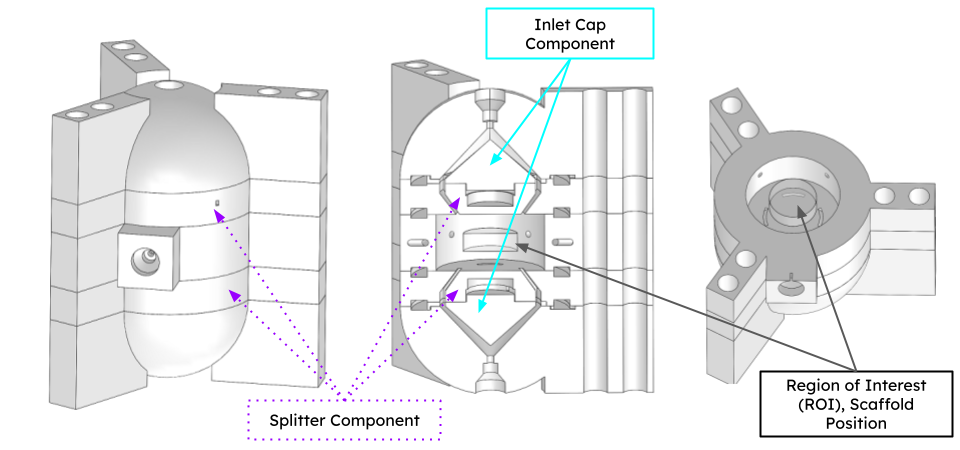
\includegraphics[scale=0.5]{./figures/Figure_3d3}}
\caption{Optimized bioreactor design. (A) Full view of the bioreactor exterior; (B) Vertical slice illustrating the bioreactor
interior; (C) Horizontal slice showing the \ac{ROI}. The blue and purple arrows identify components under optimization, while
the \ac{ROI} is identified by the black arrows.}
\label{fig3d3}
\end{figure} 




\section{Results}


\subsection{Modelling osteogenic promoting perfusion flow}

Several inlet velocities were tested to find a combination of inlet and outlet flow conditions to originate a flow range in the \ac{ROI} similar to the one reported in Zhao \textit{et al.} \cite{Zhao2018-ci}. \ac{FEM} results conduced to an inlet velocity of 0.003 \si{\meter\per\second} at each bioreactor inlet, combined with an outlet constant pressure value of one atmosphere. The laminar flow study predicted an average velocity of \num{1.14d-4} \si{\meter\per\second} and an average pressure of 0.6 \si{\pascal}, generating a flow of 2.58 \si{\milli\liter\per\minute} in the \ac{ROI}, which is within the considered range of 0.5 to 5 \si{\milli\liter\per\minute} used for obtaining maximum mineralization in bone tissue engineering, according to the work performed by Zhao \textit{et al.} \cite{Zhao2018-ci}. Velocity and pressure distributions predicted inside the bioreactor model are presented in Figure \ref{figResultsA}.

\begin{figure}
\makebox[\textwidth][c]{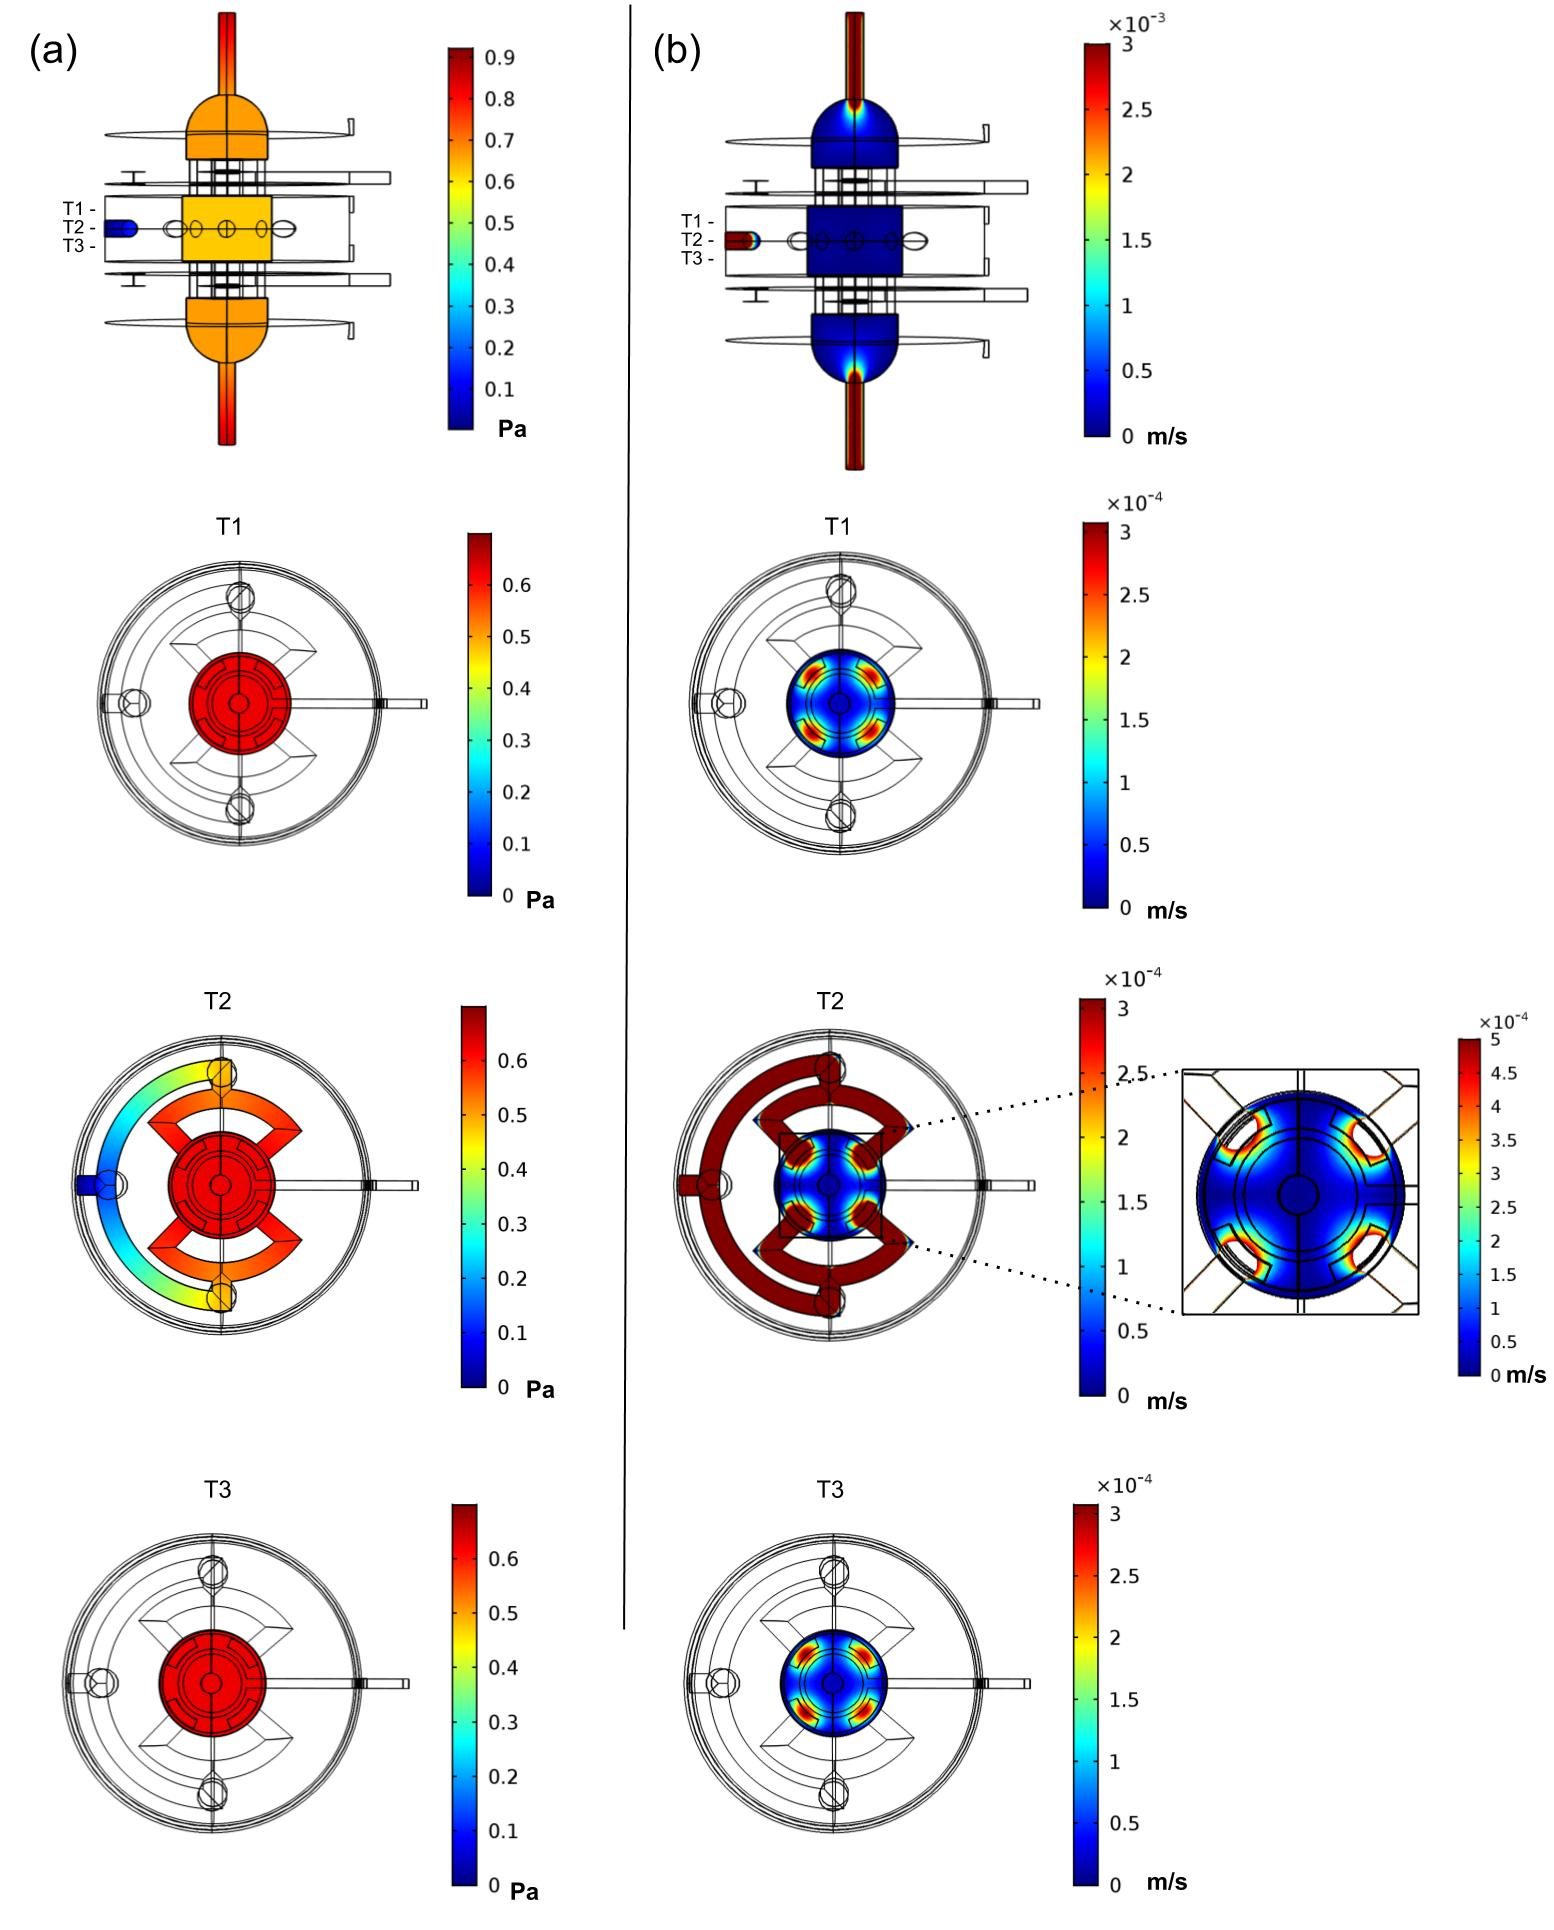
\includegraphics[scale=0.22]{./figures/Figure_3d4}}
\caption{\ac{FEM} analysis of the proposed bioreactor design for a laminar perfusion flow with lateral (upper row) and top slice views. The three top views represent the \ac{ROI} upper slice (T1), the \ac{ROI} middle plane slice (T2), and the ROI bottom slice (T3).  (\textbf{a}) Pressure distribution predicted considering applied inlet velocity of 0.003 \si{\meter\per\second} and outlet pressure of one atmosphere. (\textbf{b}) Fluid velocity distribution predicted for the same inlet/outlet conditions. The velocity distribution at the \ac{ROI} middle plane slice is presented in more detail in a top-view inset at the right of the slice plane.}
\label{figResultsA}
\end{figure}


\subsection{Adapting perfusion bioreactor design to limiting hardware}

\textit{Inlet cap component optimization.} The main goal was to reduce the flow velocity loss at the output of this component. For this purpose, three design hypotheses were tested (Figure \ref{figInlet}): (E) initial design starting point; (F) size reduction applied to all output channels; (G) pyramidal fill added to design hypothesis F. This design hypothesis were created considering that progressively directing the inlet flow to the output channels through a shorter path would lead to higher velocities. \ac{FEM} analyses were run independently for the three inlet component hypotheses. Hypothesis G was predicted to be the most suitable design for the established goal, since it increased the outflow average velocity to 0.0021 \si{\meter\per\second} per channel (26 times less than the bioreactor inlet velocity), in comparison to the design hypothesis E, where the outflow average velocity was predicted to be 50 times less than the bioreactor inlet velocity (Figure \ref{figInletResult}). Compared with design hypothesis F, design G results in the same outflow average velocity, but it requires less fluid to operate, which is an advantage in \ac{TE} applications due to the costs of the cell culture medium. Therefore, design G was chosen because it improves outflow average velocity and reduces liquid volume requirement.

\begin{figure}
\makebox[\textwidth][c]{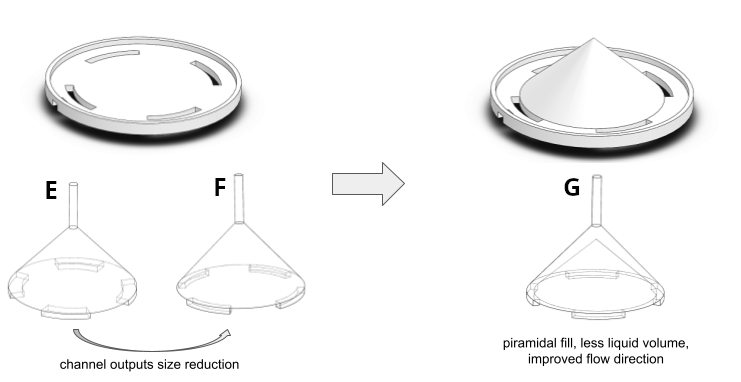
\includegraphics[scale=0.55]{./figures/Figure_3d5}}
\caption{Inlet component optimization: illustration of design hypotheses E, F, and G.}
\label{figInlet}
\end{figure}

\begin{figure}
\makebox[\textwidth][c]{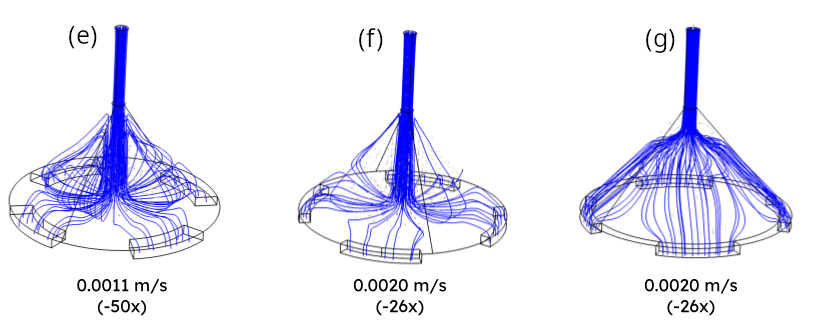
\includegraphics[scale=0.5]{./figures/Figure_3d6}}
\caption{Inlet component optimization: streamlines representing the fluid flow for each design hypothesis. The estimated
average outflow velocity and the number of times above the inlet velocity are indicated below in parentheses.}
\label{figInletResult}
\end{figure} 


\textit{Splitter component optimization.} For this component and augmented bioreactor dimensions, the main goal was to obtain the generated fluid flow-induced \ac{WSS} in the \ac{ROI} within the range of 0.11 - 60 \si{\milli\pascal}, as determined previously by Zhao \textit{et al.}, since this \ac{WSS} range was observed to effectively promote osteogenic differentiation and improve bone matrix secretion \cite{Zhao2018-ci}. First, the inlet component design shown in Figure \ref{figInlet}c was assumed as part of the bioreactor. Then, the entire liquid volume was filled, and the cylindrical \ac{ROI} was placed in the middle of the bioreactor. Four design hypotheses were tested, each assuming design variations in channel size and configuration that will originate different fluid flow velocities and directions. The tip of the channel size was progressively decreased, and its direction is progressively pointed towards the \ac{ROI} (Figure \ref{figSplitter}). Channel sizes hypothesis: A - 3.86 \si{\milli\meter}; B - 2.00 \si{\milli\meter}; C - 1.50 \si{\milli\meter}; D - 1.00 \si{\milli\meter}. For Newtonian fluids, shear stress $(\tau_s)$ is related to the shear rate $(\tau_r)$, calculated with COMSOL, by using the kinematic viscosity $(\mu)$ with the following equation \ref{TAU}.

\begin{equation}
\label{TAU}
\tau_r = \tau_s/\mu
\end{equation}

Using this equation \ref{TAU}, the shear rate values should lie in the range of 0.15 - 86 \si{\per\second}, corresponding to a \ac{WSS} range of 0.11 - 60 \si{\milli\pascal} at the \ac{ROI} as pointed by Zhao \textit{et al.} \cite{Zhao2018-ci}. Design hypothesis D was predicted to have the most considerable average shear rate at the \ac{ROI} within the range determined above, with a mean value of 0.30 \si{\per\second} (max:0.71 \si{\per\second}, min:0.046 \si{\per\second}), thus it was considered to be the best splitter component to achieve the proposed goals for mechanical stimulation inside optimal osteoinductive ranges.

\begin{figure}
\makebox[\textwidth][c]{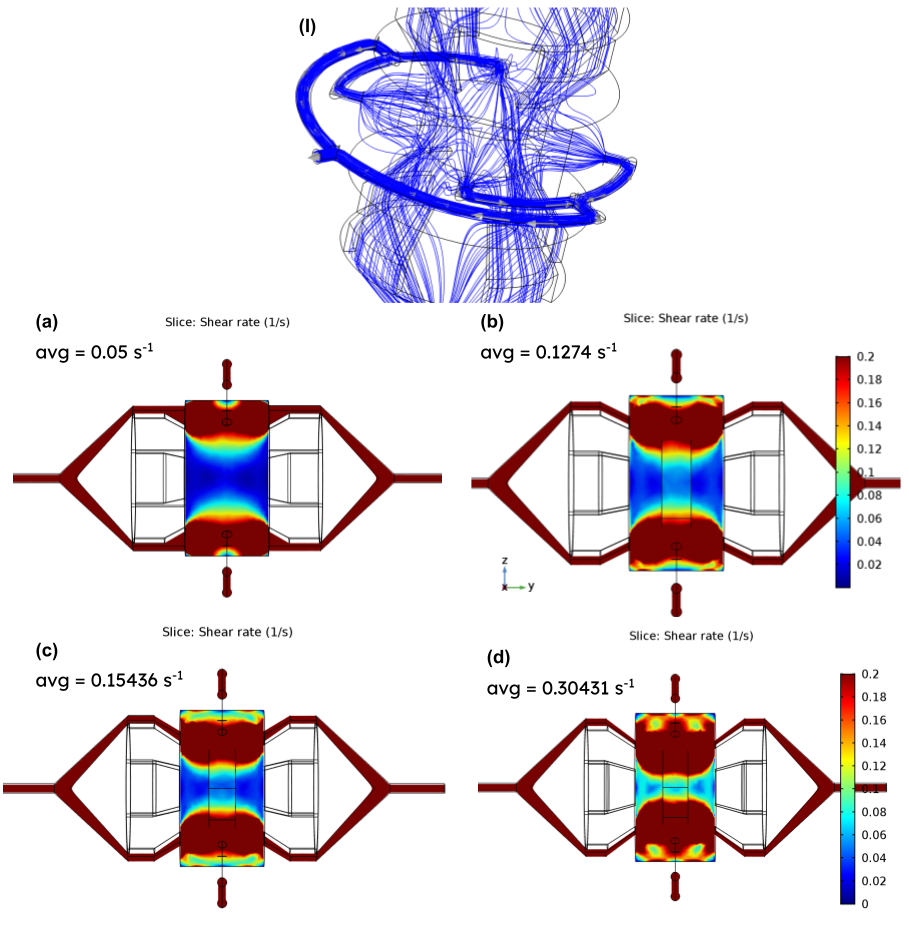
\includegraphics[scale=0.45]{./figures/Figure_3d7}}
\caption{(i) Shows the \ac{CFD} streamline plot for the center of the bioreactor, including a perspective over the outlet radial channels. Splitter component optimization: computer fluid dynamics results for fluid shear rate (1/s). The predicted shear rate average (avg) at the \ac{ROI} was calculated for each design hypothesis and is indicated below each figure index letter. Each channel end size tested hypothesis: (a) 3.86 \si{\milli\meter}; (b) 2.00 \si{\milli\meter}; ((c) 1.50 \si{\milli\meter}; (d) 1.00 \si{\milli\meter}.}
\label{figSplitter}
\end{figure} 




\section{Discussion}
This work demonstrated that applying a well-established \ac{CFD} numerical model is critical to predict and design the flow outcomes of a perfusion bioreactor. \ac{CFD} equations can be applied to predict fluid velocity, shear stress, and pressure stimulation conditions at the cell culture region and at other regions of the developed perfusion bioreactor design. These \ac{CFD} models can help find the input conditions needed to obtain or replicate a determined microenvironment in a custom design, like in the bioreactor proposed. Additionally, to adapt a protocol for a particular design, \ac{CFD} numerical models can be interactively used to shape and redesign parts or expand designs, generate specific mechanical stimulation hypotheses, or accommodate existing laboratory equipment that may constrain perfusion.  

Although empty chamber \ac{CFD} model predictions are adequate to compare different perfusion setups, introducing a cell culture scaffold will affect how the fluid flows. Thus, \ac{FEM} studies should consider the scaffold geometry to find the appropriate inlet/outlet conditions for each specific scaffold, a subsequently conducted study that its described in Chapter 6. The mechanical stimulation systems that act through fluidic interactions need to take into account the geometry of the scaffold once it creates different stimulation regions by shaping the microfluidic dynamics, as observed by Porter \textit{et al.} \cite{Porter2005-fd}, and predicted numerically by others \cite{Seddiqi2020-ti, Saatchi2020-bg}. In an original approach, Li \textit{et al.} \cite{Li2009-wu} manipulated fluid flow velocity and viscosity (by using dextran concentration) to be able to treat fluid flow-induced shear stress and mass transport as independent variables. They observed that, for $\beta$-tricalcium phosphate scaffolds seeded with \ac{MSCs}, that increasing flow-induced shear stress accelerated osteogenic differentiation and improved mineralization, while increased mass transport inhibited \ac{ECM} mineralization. The \ac{CFD} models proposed in this chapter were recently applied by Capuana \textit{et al.} \cite{Capuana2023-ik} to an airlift perfusion bioreactor in two stages: first, considering the entire bioreactor apparatus with a scaffold support multigrid; second, considering a micro-computed tomography of a region of a \acs{PLLA} scaffold produced by thermally induced phase separation. They confirm their two-step numerical predictions as essential to understand the turbulent characteristics generated by their developed bioreactor. Our bioreactor design concepts are conceived to create laminar flow conditions, reducing the numerical model's complexity and thus reinforcing the confidence in the numerical predictions. Posteriorly, adding scaffold structures, performing the cell seeding process, and even cell proliferation, growth, and external cellular matrix secretion will impact how fluid flows and the resultant shear stress is delivered to cells. This phenomenon needs to be further addressed.  

To fully take advantage of \ac{CFD} models' potential, these must be validated for each bioreactor/scaffold design combination, considering the limitations imposed by existing laboratory equipment. Validated models could then be applied to control, update, and optimize mechanical stimulation conditions in real-time \cite{Post2022-pr}. Also, refining mechanical stimulation protocols and their delivery may improve the understanding of cellular mechanotransduction responses.



\section{Summary}
This chapter proposes a novel design of a perfusion bioreactor for \ac{BTE} \textit{in vitro} applications. This design allows the application of fluid flow-induced shear stress aiming at more significant outcomes in cell differentiation, migration, and proliferation with bone cell lines. It also underlines the importance of combining \ac{3D} \ac{CAD} design and \ac{CFD} numerical modelling simulations to find the optimal input that generates the desired stimulation ranges, informed by previous experimental studies, and to optimize outcomes for \ac{TE} purposes. A data-driven design approach based on numerical predictions will be essential to create and optimize experimental conditions to understand the underlying biophysical effects of mechanical stimuli in cell cultures. It can be a powerful tool for standardizing stimulation protocols considering different bioreactor designs, diverse lab equipment, and specific BTE outcomes. The CFD framework applied here will be further explored in Chapter 6, where all individual numerical models were combined into a multimodal stimulation bioreactor design strategy.  


%\newpage
%\bibliography{library_c3b} 
%\bibliographystyle{plain}
%\end{document}